\section{Memory Management}

	% Section overview.
	In this section, we detail the internals of the memory management
	subsystem. We first present the memory layout of a process in
	Nanvix, then we introduce the memory region abstraction, and finally
	we detail the virtual memory and paging systems.

\subsection{Memory Layout}
\label{subsection: memory layout}

	% Memory layout overview.
	The virtual memory layout of typical process in Nanvix is presented
	in Figure \ref{figure: virtual memory layout}. The overall address
	space is divided in two great portions: one that is owned by the
	kernel and is shared among all processes; and a second one that is
	private and belongs to the process itself. The kernel is the only
	one that has full access to the address space of a process. While
	running in user mode, if a process touches any kernel memory, a
	protection fault is raised. This way, the kernel can isolate and
	protect itself against malicious software, thus increasing the
	system's security and reliability.

	\begin{figure}[!b]
		\centering
		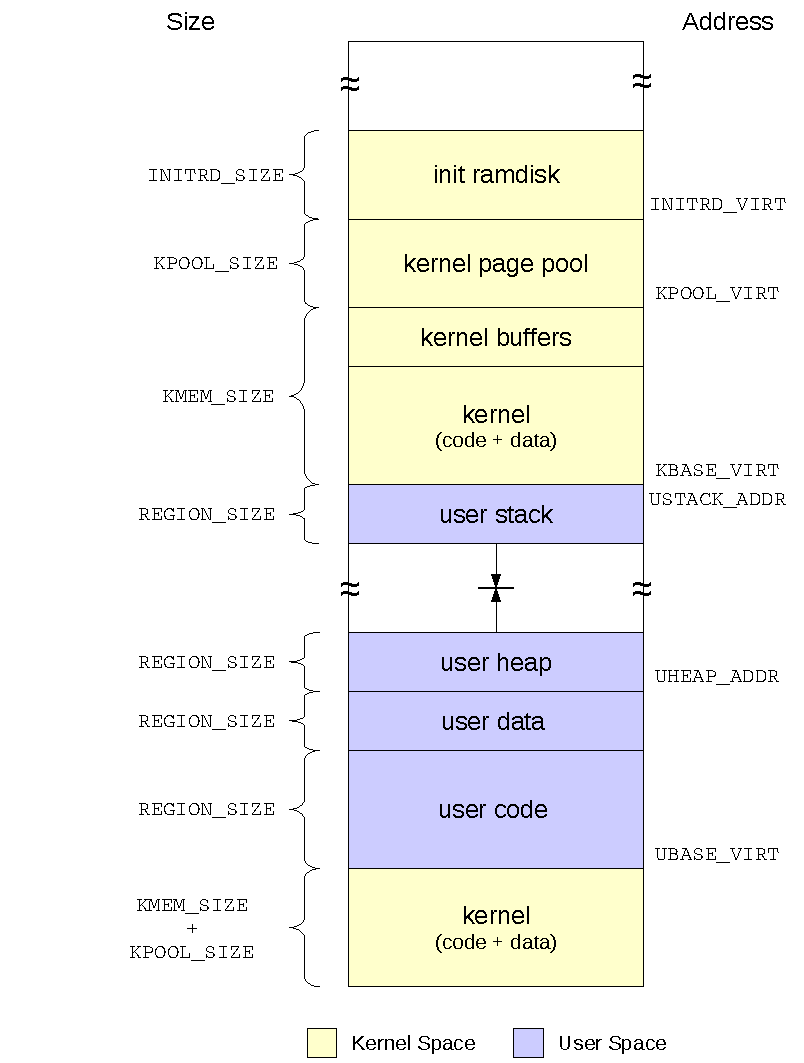
\includegraphics[scale=0.60]{img/memory-layout}
		\caption{Virtual memory layout of a process in Nanvix.}
		\label{figure: virtual memory layout}
	\end{figure}

	% Kernel code and data segments.
	The kernel address space is carefully handcrafted so that it looks
	as transparent as possible to user processes. The kernel code and
	data segments are placed to two different locations: identity mapped
	at the bottom of the memory, and virtually linked just after the
	user memory. Some operations performed by the kernel, like physical
	memory copy and context switching, require the virtual memory system
	to be shutdown momentarily. Placing the kernel code and data
	segments at the bottom of the memory, enables physical address
	access; whereas positioning the whole kernel just after user memory
	ensures that future enhancements on the kernel will not affect the
	user memory layout.

	% Kernel buffers, kernel page pool init ramdisk.
	The kernel buffers, kernel page pool and init ramdisk are accessed
	exclusively through virtual addresses. The kernel buffer area
	provides the file system with some temporary memory to hold disk
	data. The kernel page pool feeds the kernel memory allocator with
	some memory that will indeed be used to build dynamic structures in
	the kernel, such as page tables. Finally, the init ramdisk is a
	static memory area that functions as an in-memory file system and
	stores configuration files and (eventually) dynamic loadable
	drivers, which are all used during system's startup.

	% User memory layout.
	The user memory portion occupies most of the virtual address space
	and it is divided in several regions. The user code and data regions
	are statically allocated and hold the text and static data segments
	of the binary file, respectively. The user stack and heap regions on
	the other hand, dynamically grow and shrink with the course of time.
	The former is used to store temporary variables and it is managed by
	the kernel's memory management subsystem. The heap region however,
	holds long-term variables and it is handled by the process itself.
	User libraries rely on the \texttt{brk()} system call to request the
	kernel to attach, or detach, some memory to the heap.

\subsection{Memory Regions}

	\begin{figure}[!b]
		\centering
		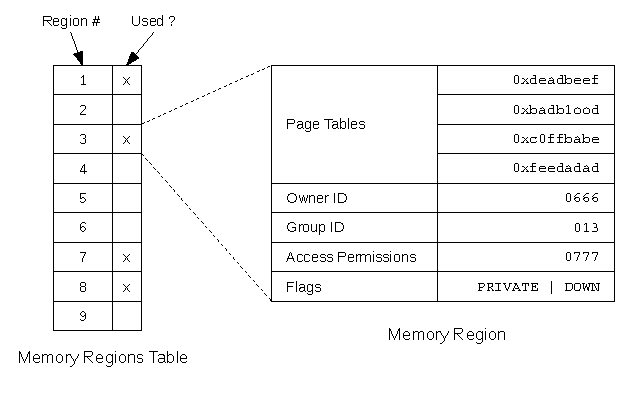
\includegraphics[scale=0.95]{img/memory-regions}
		\caption{Memory region.}
		\label{figure: memory region}
	\end{figure}

	% Memory regions in a nutshell.
	In Section \ref{subsection: memory layout} we have briefly discussed
	that the user memory portion of a process is divided in four
	regions, namely code, data, stack and heap regions. A region is a
	high-level abstraction created by the memory subsystem to easy the
	management of user memory and abstract away the underlying technique
	that is used to actually enable virtual memory (\ie segmentation or
	paging). This abstraction is presented in Figure \ref{figure: memory
	region} and briefly discussed bellow.

	% Memory regions in a paging system.
	From a design perspective, a memory region is indeed a collection of
	page tables\footnote{The memory region abstraction equally applies
	to segmentation.}, with some extra metainformation about the region
	itself. Pointers to underlying page tables are stored in a table, so
	that the virtual memory and paging systems can quickly retrieve
	low-level information about the pages that are assigned to a region.
	The owner and group IDs, and access permissions fields are used
	together to determine what processes can read or write to the memory
	region. Finally, the flags field indicate the growing direction of
	the region, whether or not the region can be swapped out to disk,
	and whether or not the region is shared among several processes.

	% Provided interface #1.
	The memory management subsystem maintains memory regions in a global
	table, namely the memory regions table, and exports a well defined
	interface for dealing with them. The process management subsystem
	heavily relies on the routines provided by this interface to
	implement the \texttt{brk()}, \texttt{exec()}, \texttt{exit()} and
	\texttt{fork()} system calls, as it is outlined in Figure
	\ref{figure: memory regions interface}. The \texttt{allocreg()}
	allocates a new memory region, by searching an empty slot in the
	memory regions table and properly initializing its fields. It is
	important to point out however, that underlying pages are not
	actually assigned to the memory region in this routine, but they are
	rather allocated on-the-fly, using a technique called demand paging
	(see Section \ref{subsection: the virtual memory and paging
	systems}). Conversely, \texttt{freereg()} frees a region table by
	releasing underlying pages and page tables, and erasing the
	corresponding entry from the memory regions table.

	% Provided interface #2.
	The \texttt{loadreg()} routine is used to load a region with some
	data from a binary file. This routine invokes raw I/O procedures
	exported by the file system to actually find the corresponding inode
	and perform the read operation. The \texttt{growreg()} procedure
	expands (or shrinks) a target region by a certain size, by
	allocating/freeing page tables accordingly. The \texttt{attachreg()}
	and \texttt{detachreg()} routines attach and detach a memory region
	to the address space of a process, respectively. They do so by
	effectively linking/unlinking underlying page tables to/from the
	page directory of a process. Finally, the \texttt{dupreg()} routine
	creates an exact copy of a target memory region. To speedup this
	task, the memory management subsystem uses a lazy copying technique
	known as copy-on-write, which e further discuss in Section
	\ref{subsection: the virtual memory and paging systems}.

	\begin{figure}[!t]
		\centering
		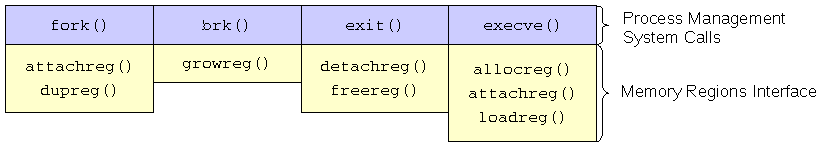
\includegraphics[scale=0.8]{img/memory-regions-interface}
		\caption{Memory regions interface.}
		\label{figure: memory regions interface}
	\end{figure}

\subsection{The Virtual Memory and Paging Systems}
\label{subsection: the virtual memory and paging systems}

	% Virtual memory system overview.
	While the memory management system exports the memory region
	interface to other system modules, internally it works with paging
	and swapping to enable virtual memory. The former technique delivers
	a flat memory abstraction, whereas the latter effectively enables
	the physical memory to be virtually extended.

	% Paging system overview.
	The paging system relies on a two-level page table that is depicted
	in Figure \ref{figure: paging scheme} and detailed next. Each
	process has a single page directory, and each entry in this
	directory points to a page table. Whenever a virtual address is
	generated, the memory management unit (MMU) breaks it in three
	portions. The upper portion is used to index the currently active
	page directory, and thus to find out the corresponding page table.
	Then, the middle portion is used to index the page table, and hence
	to discover the physical frame where the requested page is placed.
	Finally, the third portion is added to the address of the memory
	frame to build the ultimate target physical address.

	\begin{figure}
		\centering
		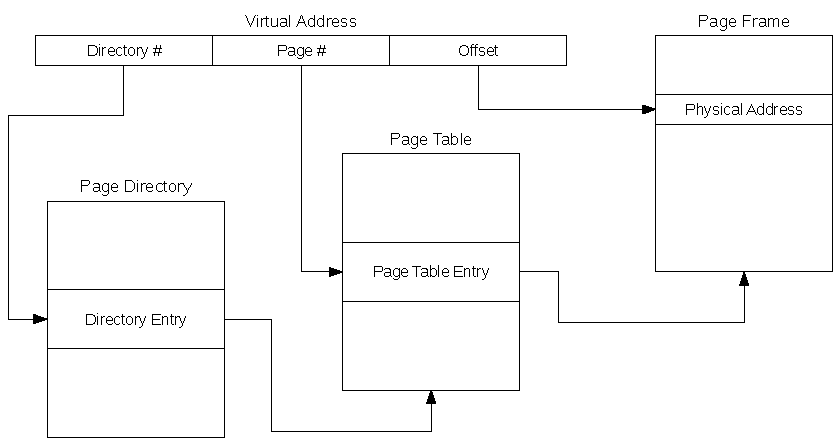
\includegraphics[scale=0.85]{img/paging-scheme}
		\caption{Two-level paging scheme used in Nanvix.}
		\label{figure: paging scheme}
	\end{figure}

	% Paging system internals.
	Page directories and page tables of all processes are pinned down in
	kernel memory, and the paging system carefully bookkeeps the
	physical addresses of these structures. This way, the kernel can
	access any address space from whatever process is running, handle
	physical memory copying, and step away from live locks when
	performing swapping. Memory frames, on the other hand, are handled
	in a different way by the internal memory frame allocator. The
	paging system maintains a table, namely the memory frames table,
	where all information about in-memory pages are stored. When the
	system first startups, it marks all entries in this table as not
	used. Whenever a page is requested, the paging system searches this
	table for an empty slot and allocates the corresponding memory
	frame. If no slot is available, the swapping system is invoked to
	swap out an in-memory page to disk.

	% Demand paging.
	Aside from managing page directories and page tables, and dealing
	with page allocation, it is worthy to note that the paging system
	also implements two fundamental mechanisms: demand paging and
	copy-on-write. The former is extensively used in the \texttt{exec()}
	system call and works as follows. Whenever an executable file needs
	to be loaded to memory, the paging system does not copy any data
	from disk nor allocate any space in memory at first. Instead, it
	marks all corresponding entries in the page table as ``not present,
	demanded paging''. Later, when an attempt to access an address that
	falls in such kind of page is made, a page fault occurs and then the
	paging system allocates a frame to that page and loads it in to
	memory. 

	% Copy-on-write.
	The second mechanism, namely copy-on-write, is heavily employed in
	the \texttt{fork()} system call to easy the overall task of creating
	a new process. In a nutshell, this system call creates a child
	process that is an exact copy of the calling process by duplicating
	every opened file descriptor and cloning the memory address space of
	the parent process. The former step can be completed in a handful of
	time as it comes down to iterate over the file descriptors table
	incrementing the reference count for each opened file. On the other
	hand, cloning the address space of a process can be a real
	time-consuming endeavor, since that involves copying a massive
	amount of data. When copy-on-write is enabled however, such
	operation is greatly speed up by having the copy operation to happen
	on demand, rather than immediately. To enable so, at first, the
	kernel marks writable pages of the parent process as ``read-only,
	copy-on-write''. Later, when a write attempt is made to a marked
	page, a protection fault is fired and the kernel performs the actual
	cloning, marking both pages as writable in the end.

	% Swapping system overview.
	So far, we have detailed the internals of the paging system, which
	delivers a flat memory abstraction to the whole system, but now it
	is time to turn our attentions to the swapping system. The ultimate
	goal of this later one is to keep in memory those pages that are
	more frequently used, and use some disk space to store those that
	are not. This way, it is possible to execute a process whose memory
	footprint is larger than the physical memory available. In other
	words, the physical memory is virtual extended, enabling the maximum
	memory footprint of a process to be bounded by the size of the
	virtual address space, rather than the physical one.

	% Page eviction.
	To achieve such goal, the swapping system relies on a
	First-in-First-out (FiFo) strategy to evict pages to disk. For each
	in-memory page, the swapping system bookkeeps the timestamp in which
	that page has been brought into memory. Whenever the swapper is
	invoked, the page with the oldest timestamp is evicted to the
	swapping area, in disk. The swapping system selects pages using a
	local-policy and implements no load control mechanism. On the other
	way around, when a page is brought in to memory from the swapping
	area, a shadow copy is kept there. This way, if no modifications are
	done to that page, no extra I/O operation to write the page back to
	disk needs to be performed.
